\documentclass[11pt]{article}
\title{Symmetry 9}
\author{https://github.com/heptagons/lenses}
\date{2024/1/14}

\usepackage{graphicx}

\usepackage[margin=0.75in]{geometry}
\usepackage{float} % {figure}{H}
\usepackage{amsmath} % \dfrac

\def\mathbi#1{\textbf{\em #1}}

\begin{document}

\maketitle
\begin{abstract}
Symmetry 9
\end{abstract}

\section{Rhombi}

\begin{table}[H]
\begin{center}
\begin{tabular}{|c|c|c c| r |}
\hline
Rhombus & Name & $\theta_1$ & $\theta_2$ & Area \\ \hline\
$R_3(\frac{1}2,1)$ & $\mathbi{a}$ & $\alpha/2$ & $2\alpha/2$  & $\sin(\alpha) \approx 0.866$ \\[0.5ex]
\hline
$R_5(\frac{1}2,2)$ & $\mathbi{b}$ & $\beta/2$  & $4\beta/2$   & $\sin(2\beta) \approx 0.587$\\[0.5ex]
$R_5(1,\frac{3}2)$ & $\mathbi{c}$ & $2\beta/2$ & $3\beta/2$   & $\sin(\beta) \approx 0.951$\\[0.5ex]
\hline
$R_7(\frac{1}2,3)$ & $\mathbi{d}$ & $\gamma/2$ & $6\gamma/2$  & $\sin(3\gamma) \approx 0.433$\\[0.5ex]
$R_7(1,\frac{5}2)$ & $\mathbi{e}$ & $2\gamma/2$ & $5\gamma/2$ & $\sin(\gamma) \approx 0.781$\\[0.5ex]
$R_7(\frac{3}2,2)$ & $\mathbi{f}$ & $3\gamma/2$ & $4\gamma/2$ & $\sin(2\gamma) \approx 0.974$\\[0.5ex]
\hline
$R_9(\frac{1}2,4)$ & $\mathbi{g}$ & $\delta/2$ & $8\delta/2$  & $\sin(4\delta) \approx 0.342$\\[0.5ex]
$R_9(1,\frac{7}2)$ & $\mathbi{h}$ & $2\delta/2$ & $7\delta/2$ & $\sin(\delta) \approx 0.642$\\[0.5ex]
$R_9(\frac{3}2,3)$ & $\mathbi{a}$ & $3\delta/2$ & $6\delta/2$ & $\sin(3\delta) \approx 0.866$\\[0.5ex]
$R_9(2,\frac{5}2)$ & $\mathbi{i}$ & $4\delta/2$ & $5\delta/2$ & $\sin(2\delta) \approx 0.984$\\[0.5ex]
\hline
\end{tabular}
\caption{Rhombi for symmetries $\{3,5,7,9\}$ internal angles $\theta_1 < \theta_2$ ($\theta_1 + \theta_2 = \pi$) and areas. $\alpha = 2\pi/3$, $\beta = 2\pi/5$, $\gamma = 2\pi/7$ and $\delta = 2\pi/9$ $(3\delta = \alpha)$.} 
\label{tbl:rhombi}
\end{center}
\end{table}

\begin{table}[H]
\begin{center}
\begin{tabular}{|c|c|l|l|}
\hline
Star & Name & Area & Polygon \\ \hline\
$S_3(\frac{1}2,1)$ & -     & $6\mathbi{a}$ & $|6/2|$ hexagram \\[0.5ex]
$S_3(1,1)$ & $\mathcal{A}$ & $3\mathbi{a}$ & Regular hexagon \\[0.5ex]
\hline
$S_5(\frac{1}2,4)$ & -      & $5\mathbi{b}$ & $|10/4|$ decagram\\[0.5ex]
$S_5(1,3)$ & $\mathcal{B}$ & $5\mathbi{c}$ & $|(5/2)_\alpha|$ decagram\\[0.5ex]
$S_5(2,2)$ & $\mathcal{C}$ & $5(\mathbi{c}+\mathbi{b})$ & Regular decagon\\[0.5ex]
\hline
$S_7(\frac{1}2,6)$ & -     & $7\mathbi{d}$ & $|14/6|$ 14-gram\\[0.5ex]
$S_7(1,5)$ & $\mathcal{D}$ & $7\mathbi{e}$ & $|(7/4)_\alpha|$ 14-gram\\[0.5ex]
$S_7(2,4)$ & $\mathcal{E}$ & $7(\mathbi{e}+\mathbi{f})$ & $|(7/2)_\alpha|$ 14-gram\\[0.5ex]
$S_7(3,3)$ & $\mathcal{F}$ & $7(\mathbi{e}+\mathbi{f}+\mathbi{d})$ & Regular 14-gon\\[0.5ex]
\hline
$S_9(\frac{1}2,7)$ & -     & $9\mathbi{g}$ & $|18/8|$ 18-gram\\[0.5ex]
$S_9(1,6)$ & $\mathcal{G}$ & $9\mathbi{h}$ & $|(9/6)_\alpha|$ 18-gram\\[0.5ex]
$S_9(2,5)$ & $\mathcal{H}$ & $9(\mathbi{h}+\mathbi{i})$ & $|(9/4)_\alpha|$ 18-gram\\[0.5ex]
$S_9(3,4)$ & $\mathcal{I}$ & $9(\mathbi{h}+\mathbi{i}+\mathbi{a})$ & $|(9/2)_\alpha|$ 18-gram\\[0.5ex]
$S_9(4,4)$ & $\mathcal{J}$ & $9(\mathbi{h}+\mathbi{i}+\mathbi{a}+\mathbi{g})$ & Regular 18-gon\\[0.5ex]
\hline
\end{tabular}
\caption{Stars $\{\mathcal{A},\mathcal{B},...\mathcal{J}\}$ for symmetries $\{3,5,7,9\}$.}
\label{tbl:stars}
\end{center}
\end{table}


\subsection{Stars from rhombi}

\begin{figure}[H]
\centering
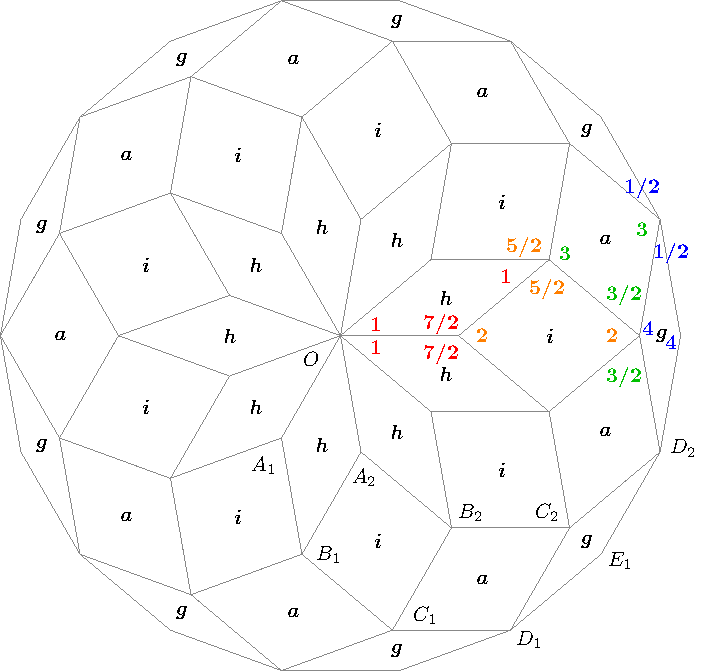
\includegraphics[scale=1]{rhombi-9}
\caption{The symmetry $9$ four rhombi $\{\mathbi{h},\mathbi{i},\mathbi{a},\mathbi{g}\}$ produce the four stars $\{\mathcal{G},\mathcal{H},\mathcal{I},\mathcal{J}\}$ with areas
$9\mathbi{h}$,
 $9(\mathbi{h}+\mathbi{i})$,
 $9(\mathbi{h}+\mathbi{i}+\mathbi{a})$ and 
 $9(\mathbi{h}+\mathbi{i}+\mathbi{a}+\mathbi{g})$ respectivelly.}
\label{fig:rhombi-9}
\end{figure}

Figure \ref{fig:rhombi-9} show nine copies of symmetry-9 rhombi $\{\mathbi{h},\mathbi{i},\mathbi{a},\mathbi{g}\}$ to form four stars.




\section{Hexagons}

\subsection{Hexagons from stars}

\begin{figure}[h]
\centering
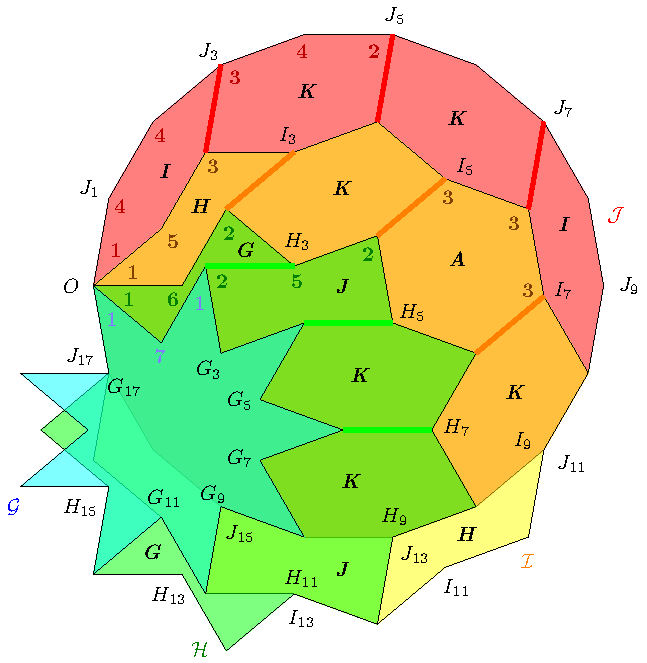
\includegraphics[scale=1]{hexagons-9}
\caption{Symmetry $9$ stars $\{\mathcal{G},\mathcal{H},\mathcal{I},\mathcal{J}\}$
 dissected to get the six hexagons
$\{\mathbi{G},\mathbi{H},\mathbi{I},\mathbi{J},\mathbi{K},\mathbi{A}\}$.
}
\label{fig:hexagons-9}
\end{figure}

Figure \ref{fig:hexagons-9} show the disposition of the symmetry $9$ four stars. We denote the $18$ vertices of stars $\{\mathcal{G},\mathcal{H},\mathcal{I},\mathcal{J}\}$ as
 $\{G_0,G_1,...,G_{17}\}$,
 $\{H_0,H_1,...,H_{17}\}$,
 $\{I_0,I_1,...,I_{17}\}$ and
 $\{I_0,G_1,...,I_{17}\}$ respectivelly. 
For simplification only some vertices are labeled in the figure. First we make coincident at vertice $O$ all the vertices $G_0,H_0,I_0,J_0$. With the center at $O$ we rotate all stars to make coincidents
$G_{17}$, $H_{17}$, $I_{17}$ and $J_{17}$. The rotations also joined another different vertices.

First we add three new edges (in red) joining the stars $\mathcal{J}$ and $\mathcal{I}$ vertices: $\overline{J_3I_2}$, $\overline{J_5I_4}$ and $\overline{J_7I_6}$ dissecting the red region into four hexagons, two of them essentially different. The three consective angles of the two hexagons are shown: $\textbf{I (1,4,4)}$ and $\textbf{K (3,4,2)}$.

Then we add three new edges (in orange) joining the stars $\mathcal{I}$ and $\mathcal{H}$ vertices: $\overline{I_3H_2}$, $\overline{I_5H_4}$ and $\overline{I_7H_6}$ dissecting the orange region into four hexagons, two of them new. The three consective angles of the the two hexagons are show: $\textbf{H (1,5,3)}$ and $\textbf{A (3,3,3)}$.

Finally we add three more edges (in green) joining the stars $\mathcal{H}$ and $\mathcal{G}$ vertices:
$\overline{H_3G_2}$, $\overline{H_5G_4}$ and $\overline{H_7G_6}$ dissecting the green region into four hexagons, two of them new. The three consective angles of the the two hexagons are show: $\textbf{G (1,6,2)}$ and $\textbf{J (2,5,2)}$.




The three consecutive angles of the hexagons are of the form $(a,b,c)$ where $a+b+c = 9$. Table \ref{tbl:hexagons-angles}

\begin{table}[H]
\begin{center}
\begin{tabular}{| c | c | c | l | }
\hline
Hexagon & Name & $(\textbf{a, b, c})$ & Polygon \\ \hline\
$H_3(1,1)$ & \mathbi{A} & (\textbf{1, 1, 1}) & Regular hexagon \\[0.5ex]
\hline
$H_5(1,1)$ & \mathbi{B} & (\textbf{1, 1, 3}) & Sormeh Dan Girih tile\\[0.5ex]
$H_5(1,2)$ & \mathbi{C} & (\textbf{1, 2, 2}) & Shesh Band Girih tite\\[0.5ex]
\hline
$H_7(1,1)$ & -          & (\textbf{1, 1, 5}) & self-intersecting \\[0.5ex]
$H_7(1,2)$ & \mathbi{D} & (\textbf{1, 2, 4}) & \\[0.5ex]
$H_7(1,3)$ & \mathbi{E} & (\textbf{1, 3, 3}) & \\[0.5ex]
$H_7(2,2)$ & \mathbi{F} & (\textbf{2, 2, 3}) & \\[0.5ex]
\hline
$H_9(1,1)$ & -          & (\textbf{1, 1, 7}) & self-intersecting \\[0.5ex]
$H_9(1,2)$ & \mathbi{G} & (\textbf{1, 2, 6}) & \\[0.5ex]
$H_9(1,3)$ & \mathbi{H} & (\textbf{1, 3, 5}) & \\[0.5ex]
$H_9(1,4)$ & \mathbi{I} & (\textbf{1, 4, 4}) & \\[0.5ex]
$H_9(2,2)$ & \mathbi{J} & (\textbf{2, 2, 5}) & \\[0.5ex]
$H_9(2,3)$ & \mathbi{K} & (\textbf{2, 3, 4}) & \\[0.5ex]
$H_9(3,3)$ & \mathbi{A} & (\textbf{3, 3, 3}) & symmetry 3 hexagon\\[1.1ex]
\hline
\end{tabular}
\caption{Hexagons of symmetries $\{3,5,7,9\}$ with angles factors $\mathbf{a} \leq \mathbf{b} \leq \mathbf{c}$.} 
\label{tbl:hexagons-angles}
\end{center}
\end{table}




\end{document}

